\chapter{On the Absolute Quantity of Electricity Associated with the Particles or
Atoms of Matter}

\chapterprecis{}

\chapterprecishere{Michael Faraday\footnote{[\emph{Experimental Researches in Electricity}, 
   VIIth series, section 13. Dover edition, Vol.I, 249ff.]}}
\chapterprecistoc{Michael Faraday}


\makeoddhead{myheadings}{\emph{Faraday}}{}{\thepage}
\makeevenhead{myheadings}{\thepage}{}{\emph{On the Absolute Quantity of Electricity}}

\indent
852. The theory of definite electrolytical or electro-chemical action
appears to me to touch immediately upon the \emph{absolute quantity} of
electricity or electric power belonging to different bodies. It is
impossible, perhaps, to speak on this point without committing oneself
beyond what present facts will sustain; and yet it is equally
impossible, and perhaps would be impolitic, not to reason upon the
subject. Although we know nothing of what an atom is, yet we cannot
resist forming some idea of a small particle, which represents it to the
mind; and though we are in equal, if not greater, ignorance of
electricity, so as to be unable to say whether it is a particular matter
or matters, or mere motion of ordinary matter, or some third kind of
power or agent, yet there is an immensity of facts which justify us in
believing that the atoms of matter are in some way endowed or associated
with electrical powers, to which they owe their most striking qualities,
and amongst them their mutual chemical affinity. As soon as we perceive,
through the teaching of Dalton, that chemical powers are, however varied
the circumstances in which they are exerted, definite for each body, we
learn to estimate the relative degree of force which resides in such
bodies: and when upon that knowledge comes the fact, that the
electricity, which we appear to be capable of loosening from its
habitation for awhile, and conveying from place to place, \emph{whilst
it retains its chemical force}, can be measured out, and being so
measured out is found to be \emph{as definite in its action} as any of
\emph{those portions} which, remaining associated with the particles of
matter, give them their \emph{chemical relation}; we seem to have found
the link which connects the proportion of that we have evolved to the
proportion of that belonging to the particles in their natural state.

853. Now it is wonderful to observe how small a quantity of a compound
body is de\-com\-posed by a certain portion of electricity. Let us, for
instance, consider this and a few other points in relation to water.
\emph{One grain}\footnote{{[}One grain is about .065 grams.{]}} of
water, acidulated to facilitate conduction, will require an electric
current to be continued for three minutes and three quarters of time to
effect its de\-com\-po\-si\-tion, which current must be powerful enough to
retain a platina wire 1/104 of an inch in thickness,\footnote{I have not
  stated the length of wire used, because I find by experiment, as would
  be expected in theory, that it is indifferent. The same quantity of
  electricity which, passed in a given time, can heat an inch of platina
  wire of a certain diameter red hot, can also heat a hundred, a
  thousand, or any length of the same wire to the same degree, provided
  the cooling circumstances are the same for every part in all cases.
  This I have proved by the volta-electrometer. I found that whether
  half an inch or eight inches were retained at one constant temperature
  of dull redness, equal quantities of water were de\-com\-posed in equal
  times. When the half-inch was used, only the center portion of wire
  was ignited. A fine wire may even be used as a rough but ready
  regulator of a voltaic current; for if it be made part of the circuit,
  and the larger wires communicating with it be shifted nearer to or
  further apart, so as to keep the portion of wire in the circuit
  sensibly at the same temperature, the current passing through it will
  be nearly uniform.} red hot, in the air during the whole time; and if
interrupted anywhere by charcoal points, will produce a very brilliant
and constant star of light. If attention be paid to the instantaneous
discharge of electricity of tension, as illustrated in the beautiful
experiments of Mr. Wheatstone,\footnote{Literary Gazette, 1833, March 1
  and 8. Philosophical magazine, 1833, 204. L'Institute, 1833, 261.}
and to what I have said elsewhere on the relation of common and voltaic
electricity (371.\ 375.),\footnote{{[}Faraday refers to numbered
  paragraphs in earlier series of the \emph{Experimental Researches}.{]}}
it will not be too much to say that this necessary quantity of
electricity is equal to a very powerful flash of lightning.\footnote{{[}This
  amount of charge is indeed comparable to that in a typical lightning
  bolt.{]}} Yet we have it under perfect command; can evolve, direct,
and employ it at pleasure; and when it has performed its full work of
electrolyzation, it has only separated the elements of \emph{a single
grain of water.}

854. On the other hand, the relation between the conduction of the
electricity and the de\-com\-po\-si\-tion of the water is so close, that one
cannot take place without the other. If the water is altered only in
that small degree which consists in its having the solid instead of the
fluid state, the conduction is stopped, and the de\-com\-po\-si\-tion is stopped
with it. Whether the conduction be considered as depending upon the
de\-com\-po\-si\-tion, or not (413.\ 703.), still the relation of the two
functions is equally intimate and inseparable.

855. Considering this close and twofold relation, namely, that without
de\-com\-po\-si\-tion transmission of electricity does not occur; and, that for
a given definite quantity of electricity passed, an equally definite and
constant quantity of water or other matter is de\-com\-posed; considering
also that the agent, which is electricity, is simply employed in
overcoming electrical powers in the body subjected to its action; it
seems a probable, and almost a natural consequence, that the quantity
which passes is the \emph{equivalent} of, and therefore equal to, that
of the particles separated; i.e.\ that if the electrical power which
holds the elements of a grain of water in combination, or which makes a
grain of oxygen and hydrogen in the right pro\-por\-tions unite into water
when they are made to combine, could be thrown into the condition of
\emph{a current}, it would exactly equal the current required for the
separation of that grain of water into its elements again.

856. This view of the subject gives an almost overwhelming idea of the
extraordinary quantity or degree of electric power which naturally
belongs to the particles of matter; but it is not inconsistent in the
slightest degree with the facts which can be brought to bear on this
point. To illustrate this I must say a few words on the voltaic
pile.\footnote{By the term voltaic pile, I mean such ap\-pa\-ra\-tus or
  arrangement of metals as up to this time have been called so, and
  which contain water, brine, acids, or other aqueous solutions or
  decomposable substances (476.), between their plates. Other kinds of
  electric ap\-pa\-ra\-tus may hereafter be invented, and I hope to construct
  some not belonging to the class of instruments discovered by Volta.
  {[}Note: The voltaic pile is an instance of what we know as the
  \emph{electric battery}; and indeed Faraday also uses the term
  ``battery'' in paragraphs 858ff. below.{]}}

857. Intending hereafter to apply the results given in this and the
preceding series of Researches to a close investigation of the source of
electricity in the voltaic instrument, I have refrained from forming any
decided opinion on the subject; and without at all meaning to dismiss
metallic contact, or the contact of dissimilar substances, being
conductors, but not metallic, as if they had nothing to do with the
origin of the current, I still am fully of the opinion with Davy, that
it is at least continued by chemical action, and that the supply
constituting the current is almost entirely from that source.

858. Those bodies which, being interposed between the metals of the
voltaic pile, render it active, \emph{are all of them electrolytes}
(476.); and it cannot but press upon the attention of every one engaged
in considering this subject, that in those bodies (so essential to the
pile) de\-com\-po\-si\-tion and the transmission of a current are so intimately
connected, that one cannot happen without the other. This I have shown
abundantly in water, and in numerous other cases (402.\ 476.). If, then,
a voltaic trough have its extremities connected by a body capable of
being de\-com\-posed, as water, we shall have a continuous current through
the ap\-pa\-ra\-tus; and whilst it remains in this state we may look at the
part where the acid is acting upon the plates, and that where current is
acting upon the water, as the reciprocals of each other. In both parts
we have the two conditions \emph{inseparable in such bodies as these},
namely, the passing of a current, and de\-com\-po\-si\-tion; and this is as true
of the cells in the battery as of the water cell; for no voltaic battery
has as yet been constructed in which the chemical action is only that of
combination: \emph{de\-com\-po\-si\-tion is always included}, and is, I believe,
an essential chemical part.

859. But the difference in the two parts of the connected battery, that
is, the de\-com\-po\-si\-tion or experimental cell, and the acting cells, is
simply this. In the former we urge the current through, but it,
apparently of necessity, is accompanied by de\-com\-po\-si\-tion: in the latter
we cause de\-com\-po\-si\-tions by ordinary chemical actions (which are,
however, themselves electrical), and, as a consequence, have the
electrical current; and as the de\-com\-po\-si\-tion dependent upon the current
is definite in the former case, so is the current associated with the
de\-com\-po\-si\-tion also definite in the latter (862.\ \&c.).

860. Let us apply this in support of what I have surmised respecting the
enormous electric power of each particle or atom of matter (856.). I
showed in a former series of these Researches on the relation by measure
of common and voltaic electricity,\footnote{{[}By ``common'' electricity
  Faraday means \emph{static} electricity; while ``voltaic'' electricity
  is what is produced by the voltaic battery. Until Faraday showed their
  equivalence, it was uncertain whether the two ``electricities'' were
  same or different.{]}} that two wires, one of platina and one of zinc,
each one eighteenth of an inch in diameter, placed five-sixteenths of an
inch apart, and immersed to the depth of five eighths of an inch in
acid, consisting of one drop of oil of vitriol and four ounces of
distilled water at a temperature of about $60^{\circ}$ Fahr., and connected at
the other extremities by a copper wire eighteen feet long, and one
eighteenth of an inch in thickness,\footnote{{[}The eighteen-foot length
  of wire formed the coil of a galvanometer. See \emph{Experimental
  Researches}, Vol. I, 105.{]}} yielded as much electricity in little
more than three seconds of time as a Leyden battery\footnote{{[}``Leyden
  battery'': an array (a ``battery'') of Leyden jars.{]}} charged by
thirty turns of a very large and powerful plate electric machine in full
action (371.). This quantity, though sufficient if passed through the
head of a rat or cat to have killed it, as by a flash of lightning, was
evolved by the mutual action of so small a portion of the zinc wire and
water in contact with it, that the loss of weight sustained by either
would be inappreciable by our most delicate instruments; and as to the
water which could be de\-com\-posed by that current, it must have been
insensible in quantity, for no trace of hydrogen appeared upon the
surface of the platina during those three seconds.

861. What an enormous quantity of electricity, therefore, is required
for the de\-com\-po\-si\-tion of a single grain of water! We have already seen
that it must be in quantity sufficient to sustain a platina wire 1/104
of an inch in thickness, red hot, in contact with the air, for three
minutes and three quarters (853.), a quantity which is almost infinitely
greater than that which could be evolved by the little standard voltaic
arrangement to which I have just referred (860.\ 371.). I have endeavored
to make a comparison by the loss of weight of such a wire in a given
time in such an acid, according to a principle and experiment to be
almost immediately described (862.); but the proportion is so high that
I am almost afraid to mention it. It would appear that 800,000 such
charges of the Leyden battery as I have referred to above, would be
necessary to supply electricity sufficient to decompose a single grain
of water; or, if I am right, to equal the quantity of electricity which
is naturally associated with the elements of that grain of water,
endowing them with their mutual chemical affinity.

862. In further proof of this high electric condition of the particles
of matter, and the \emph{identity as to quantity of that belonging to
them with that necessary for their separation}, I will describe an
experiment of great simplicity but extreme beauty, when viewed in
relation to the evolution of an electric current and its decomposing
powers.

863. A dilute sulphuric acid, made by adding about one part by measure
of oil of vitriol to thirty parts of water, will act energetically upon
a piece of zinc plate in its ordinary and simple state: but, as Mr.
Sturgeon has shewn,\footnote{Recent Experimental Researches, \&c., 1830,
  74, \&c.} not at all, or scarcely so, if the surface of the metal
has in the first instance been amalgamated; yet the amalgamated zinc
will act powerfully with platina as an electromotor,\footnote{{[}``electromotor'':
  something that moves or tends to move electricity (1827).{]}} hydrogen
being evolved on the surface of the latter metal, as the zinc is
oxidized and dissolved. The amalgamation is best effected by sprinkling
a few drops of mercury upon the surface of the zinc, the latter being
moistened with the dilute acid, and rubbing with the fingers or tow so
as to extend the liquid metal over the whole of the surface. Any mercury
in excess, forming liquid drops upon the zinc, should be wiped
off.\footnote{The experiment may be made with pure zinc, which, as
  chemists well know, is but slightly acted upon by dilute sulphuric
  acid in comparison with ordinary zinc, which during the action is
  subject to an infinity of voltaic actions. See De la Rive on this
  subject, Bibliothèque Universelle, 1830, 391.}

864. Two plates of zinc thus amalgamated were dried and accurately
weighed; one, which we shall call A, weighed 163.1 grains; the other, to
be called B, weighed 148.3 grains.\footnote{{[}Or, since one grain
  equals about .065 grams, plate A weighs about 10.6 grams and plate B
  about 9.6 grams.{]}} They were about five inches long, and 0.4 of an
inch wide. An earthenware pneumatic trough was filled with dilute
sulphuric acid, of the strength just described (863.), and a gas jar,
also filled with the acid, inverted in it.\footnote{The acid was left
  during a night with a small piece of unamalgamated zinc in it, for the
  purpose of evolving such air as might be inclined to separate, and
  bringing the whole into a constant state.} A plate of platina of
nearly the same length, but about three times as wide as the zinc
plates, was put up into this jar. The zinc plate A was also introduced
into the jar, and brought in contact with the platina, and at the same
moment the plate B was put into the acid of the trough, but out of
contact with other metallic matter.

865. Strong action immediately occurred in the jar upon the contact of
the zinc and platina plates. Hydrogen gas rose from the platina, and was
collected in the jar, but no hydrogen or other gas rose from
\emph{either} zinc plate. In about ten or twelve minutes, sufficient
hydrogen having been collected, the experiment was stopped; during its
progress a few small bubbles had appeared upon plate B, but none upon
plate A. The plates were washed in distilled water, dried, and
reweighed. Plate B weighed 148.3 grains, as before, having lost nothing
by the direct chemical action of the acid. Plate A weighed 154.65
grains, 8.45 grains of it having been oxidized and dissolved during the
experiment.
\begin{figure}
  \centering
    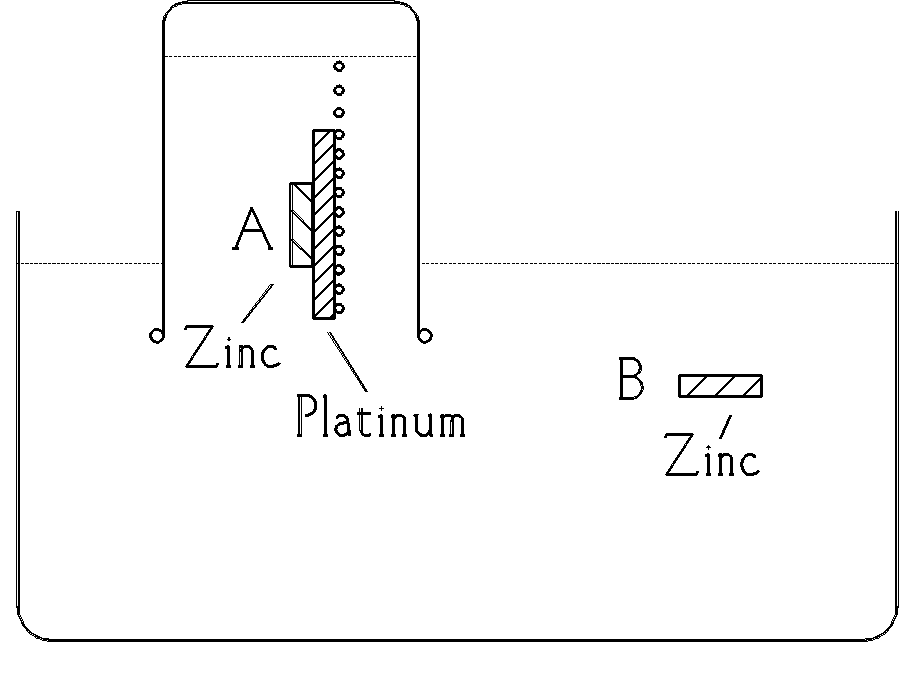
\includegraphics[width=2.68681in,height=2.00903in]{images/01_faraday/image001.png}
    \caption*{{[}A representation of Faraday's ap\-pa\-ra\-tus.{]}}
\end{figure}

866. The hydrogen gas was next transferred to a water-trough and
measured; it amounted to 12.5 cubic inches, the temperature being $52^{\circ}$,
and the barometer 29.2 inches. This quantity, corrected for temperature,
pressure, and moisture, becomes 12.15453 cubic inches of dry hydrogen at
mean temperature and pressure;\footnote{{[}Faraday uses the gas laws to
  reduce the measured volume of hydrogen to the equivalent volume at $50^{\circ}$
  F. and 30 in Hg; these are ``mean'' conditions which he takes as
  standard. The measurement is first ``corrected for moisture'' by
  subtracting the known vapor pressure of water at $52^{\circ}$ F. from the
  measured barometric pressure.{]}} which, increased by one half for the
oxygen that must have gone to the \emph{anode}, i.e.\ to the zinc, gives
18.232 cubic inches as the quantity of oxygen and hydrogen evolved from
the water de\-com\-posed by the electric current.\footnote{{[}Since
  de\-com\-po\-si\-tion of water yields hydrogen and oxygen in a 2:1 ratio by
  volume, the total volume of both gases will be 1.5 times the volume of
  hydrogen alone.{]}} According to the estimate of the weight of the
mixed gas before adopted (791.),\footnote{{[}In an earlier paragraph
  791, Faraday had reported about .129 grains per cubic inch as the
  density of a mixture of 2 volumes hydrogen and 1 volume oxygen at
  ``mean'' temperature and pressure.{]}} this volume is equal to
2.3535544 grains, which therefore is the weight of water de\-com\-posed; and
this quantity is to 8.45 {[}grains{]}, the quantity of zinc oxidized, as
9 is to 32.31. Now taking 9 as the equivalent number of water, the
number 32.5 is given as the equivalent number of zinc;\footnote{{[}The
  equivalent weight of zinc currently accepted is 32.69, about .5\%
  higher than the figure 32.5 accepted by Faraday.{]}} a coincidence
sufficiently near to show, what indeed could not but happen, that for an
equivalent of zinc oxidized an equivalent of water must be
de\-com\-posed.\footnote{The experiment was repeated several times with the
  same results.}

867. But let us observe \emph{how} the water is de\-com\-posed. It is
electrolyzed, i.e.\ is de\-com\-posed voltaically, and not in the ordinary
manner (as to appearance) of chemical de\-com\-po\-si\-tions; for the oxygen
appears at the \emph{anode} and the hydrogen at the \emph{cathode} of
the body under de\-com\-po\-si\-tion, and these were in many parts of the
experiment above an inch asunder. Again, the ordinary chemical affinity
was not enough under the circumstances to effect the de\-com\-po\-si\-tion of
the water, as was abundantly proved by the inaction on plate B; the
voltaic current was essential. And to prevent any idea that the chemical
affinity was almost sufficient to decompose the water, and that a
smaller current of electricity might, under the circumstances, cause the
hydrogen to pass to the \emph{cathode}, I need only refer to the results
which I have given (807.\ 813.), to shew that the chemical action at the
electrodes has not the slightest influence over the \emph{quantities} of
water or other substances de\-com\-posed between them, but that they are
entirely dependent upon the quantity of electricity which passes.

868. What, then, follows as a necessary consequence of the whole
experiment? Why, this: that the chemical action upon 32.31 parts, or one
equivalent of zinc, in this simple voltaic circle, was able to evolve
such quantity of electricity in the form of a current as, passing
through water, should decompose 9 parts, or one equivalent of that
substance: and considering the definite relations of electricity as
developed in the preceding parts of the present paper, the results prove
that the quantity of electricity which, being naturally associated with
the particles of matter, gives them their combining power, is able, when
thrown into a current, to separate those particles from their state of
combination; or, in other words, that \emph{the electricity which
decomposes, and that which is evolved by the de\-com\-po\-si\-tion of, a certain
quantity of matter, are alike}.

869. The harmony which this theory of the definite evolution and the
equivalent definite action of electricity introduces into the associated
theories of definite pro\-por\-tions and electro-chemical affinity, is very
great. According to it, the equivalent weights of bodies are simply
those quantities of them which contain equal quantities of electricity,
or have naturally equal electric powers; it being the
\textsc{electricity} which \emph{determines} the equivalent number,
\emph{because} it determines the combining force. Or, if we adopt the
atomic theory or phraseology, then the atoms of bodies which are
equivalent to each other in their ordinary chemical action, have equal
quantities of electricity naturally associated with them. But I must
confess I am jealous\footnote{{[}``jealous:'' here,
  \emph{suspicious}.{]}} of the term \emph{atom}; for though it is very
easy to talk of atoms, it is very difficult to form a clear idea of
their nature, especially when compound bodies are under consideration.

870. I cannot refrain from recalling here the beautiful idea put forth,
I believe, by Berzelius (703.)\ in his development of his views of the
electro-chemical theory of affinity, that the heat and light evolved
during cases of powerful combination are the consequence of the electric
discharge which is at the moment taking place. The idea is in perfect
accordance with the view I have taken of the \emph{quantity} of
electricity associated with the particles of matter.

871. In this exposition of the law of the definite action of
electricity, and its cor\-re\-spond\-ing definite proportion in the particles
of bodies, I do not pretend to have brought, as yet, every case of
chemical or electro-chemical action under its dominion. There are
numerous considerations of a theoretical nature, especially respecting
the compound particles of matter and the resulting electrical forces
which they ought to possess, which I hope will gradually receive their
development; and there are numerous experimental cases, as, for
instance, those of compounds formed by weak affinities, the simultaneous
de\-com\-po\-si\-tion of water and salts, \&c., which still require
investigation. But whatever the results on these and numerous other
points may be, I do not believe that the facts which I have advanced, or
even the general laws deduced from them, will suffer any serious change;
and they are of sufficient importance to justify their publication,
though much may yet remain imperfect or undone. Indeed, it is the great
beauty of our science, \textsc{chemistry}, that advancement in it,
whether in a degree great or small, instead of exhausting the subjects
of research, opens the doors to further and more abundant knowledge,
overflowing with beauty and utility, to those who will be at the easy
personal pains of undertaking its experimental investigation.

872. The definite production of electricity (868.)\ in association with
its definite action proves, I think, that the current of electricity in
the voltaic pile is sustained by chemical de\-com\-po\-si\-tion, or rather by
chemical action, and not by contact only. But here, as elsewhere (857.),
I beg to reserve my opinion as to the real action of contact, not having
yet been able to make up my mind as to whether it is an exciting cause
of the current, or merely necessary to allow of the conduction of
electricity, otherwise generated, from one metal to the other.

873. But admitting that chemical action is the source of electricity,
what an infinitely small fraction of that which is active do we employ
in our voltaic batteries! Zinc and platina wires, one eighteenth of an
inch in diameter and about half an inch long, dipped into dilute
sulphuric acid, so weak that it is not sensibly sour to the tongue, or
scarcely to our most delicate test papers, will evolve more electricity
in one twentieth of a minute (860.)\ than any man would willingly allow
to pass through his body at once. The chemical action of a grain of
water upon four grains of zinc can evolve electricity equal in quantity
to that of a powerful thunder-storm (868.\ 861.). Nor is it merely true
that the quantity is active; it can be directed and made to perform its
full equivalent duty (867.\ \&c.). Is there not, then, great reason to
hope and believe that, by a closer \emph{experimental} investigation of
the principles which govern the development and action of this subtile
agent, we shall be able to increase the power of our batteries, or
invent new instruments which shall a thousandfold surpass in energy
those which we at present possess?

874. Here for a while I must leave the consideration of the
\emph{definite chemical action of electricity}. But before I dismiss
this series of experimental Researches, I would call to mind that, in a
former series, I showed the current of electricity was also
\emph{definite in its magnetic action} (216.\ 366.\ 367.\ 376.\ 377.); and,
though this result was not pursued to any extent, I have no doubt that
the success which has attended the development of the chemical effects
is not more than would accompany an investigation of the magnetic
phenomena.

\begin{quotation}
\emph{Royal Institution}

\emph{December} 31\emph{st}, 1833.
\end{quotation}

\section*{A Note on Chemical Equivalence}

Faraday confesses he is ``jealous,'' that is, suspicious, of the term
\emph{atom}. When he wrote in 1833, there was no agreement among natural
philosophers as to a formula for, say, water, which would specify the
atomic constituents of a single smallest particle (mol\-e\-cule) of water:
was it HO, or H$_2$O, or something else? What Faraday \emph{was} sure of
was that chemical substances reacted in definite pro\-por\-tions by weight
and, further, that the weights of various substances reacting with one
another formed a series of ``equivalent'' or ``combining'' weights. And
since oxygen combines with so many different substances, taking oxygen
as the standard of comparison allowed indirect extension of the series
to include \emph{all} elements.

For example, 8 parts by weight of oxygen will combine with 1 part by
weight of hydrogen (to form water). But 8 parts by weight of oxygen will
also combine with 32.69 parts by weight of zinc (to form zinc oxide).
Then the 32.69 of zinc, the 8 of oxygen, and the 1 of hydrogen are all
said to be ``equivalent'' weights---equivalent, that is to say, in
\emph{combining power---}because either any two of those quantities will
combine with one another or each will combine with the specified weight
of the remaining substance. Equivalent weights are relative only to one
another and may therefore be expressed in arbitrary units of weight. But
it is particularly convenient to express them in \emph{grams}, with
\emph{8 grams of oxygen} taken as the standard. The figures so obtained
are called, not merely equivalent weights, but \emph{gram-equivalent
weights}; thus 1 gram, 8 grams, and 32.69 grams are the
\emph{gram-equivalent weights} of hydrogen, oxygen, and zinc,
respectively.

If, like Faraday, one is skeptical of the atomic view, there cannot be
assumed any natural ``unit'' of chemical combining power. Thus it is for
him illuminating in the highest degree to be able to interpret the
chemically equivalent weights of various substances as amounts which
contain ``equal quantities of electricity'' (cf.\ his paragraph 869
above).

If the atomic view is accepted, there are consequences even more
far-reaching. The molecular formulas finally propounded by Cannizzaro
(\emph{A Course in Chemical Philosophy}, 1859) show that one atom of an
element may hold in combination one, two or more atoms of other elements
by establishing an integral number of \emph{atomic bonds}, where the
bond to a hydrogen atom is taken as unit.\footnote{The number of bonds
  an atom has formed is known as its \emph{valence}. Thus in H2O (water)
  and NH3 (ammonia), the oxygen atom is said to be \emph{bivalent} and
  the nitrogen atom \emph{tervalent}. Some elements combine under
  different conditions to form more than one compound, allowing a single
  element to exhibit multiple valences. For example, a carbon atom is
  bivalent in CO but quadrivalent in CO2.

  Since ``equivalent weights'' of elements are amounts which display the
  same combining power, then on the atomic view they must also be
  amounts that form the same total number of atomic bonds. But any
  number of bivalent atoms will form as many bonds as \emph{twice} that
  number of univalent atoms; and in general, equivalent weights of
  different elements must contain numbers of atoms inversely
  proportional to their respective valences. Therefore we may state that
  \emph{the relative weights of the atoms} of different elements are as
  \emph{the products of their equivalent weights times their valences},
  respectively; or:

  Atomic weight = Equivalent weight $\times$ Valence.} Since, on the atomic
view, an atom that forms a single atomic bond manifests \emph{a natural
unit of combining power,} then under Faraday's interpretation of chemical
powers as ultimately electrical, such a unitary combining power would
appear to be associated with and perhaps even explained by \emph{a
natural unit of electricity.}

Might there really be a natural unit of electricity, an ``atom of
charge''? The papers to follow by Thomson and Millikan will bear on this
question.

\section*{Experiment: Electrodeposition of Copper}

In order to simplify the relations between chemical and electrical power
in our ap\-pa\-ra\-tus, we use a cell in which no overall chemical reaction
occurs. This is achieved by using electrodes made of the same metal as
the metal in the electrolytic solution. Under the action of electric
current metal from the positive electrode (anode) dissolves into
solution, while at the negative electrode (cathode) metal leaves the
solution and is deposited there. The net result is transfer of material
from one electrode to the other. We normally use copper electrodes, with
a copper sulfate solution as electrolyte. If available, silver
electrodes with a silver nitrate solution can be employed for comparison
with another element.\footnote{The experiment can easily be done with
  silver, provided the silver nitrate solution is protected from light;
  however the supplies are much more expensive and harder to recover
  after use.}

You may choose to weigh either the cathode, which gains material, or the
anode, which loses it. It is theoretically advantageous to weigh the
\emph{cathode}, since the anode is subject to secondary reactions in the
presence of an acid solution, producing excessive weight loss. On the
other hand, material removed from the anode may fail to adhere to the
cathode, resulting in deficient measurement of the weight gain.
Whichever your choice, results will be greatly improved if you
\emph{start with clean electrodes} and \emph{avoid excessive currents}.

The electrolyte solution is cupric sulfate dissolved in distilled water,
with the ad\-di\-tion of a small quantity of sulfuric acid, which enhances
the conductivity of the solution.

Power is furnished by a standard supply. A rheostat of about 20 ohms is
used to help regulate the current. Typically 1-2 amperes is the current
used. Higher values will require constant readjustment of the rheostat
and may cause de\-com\-po\-si\-tion of the water, as well as other problems.
\begin{figure}
\centering
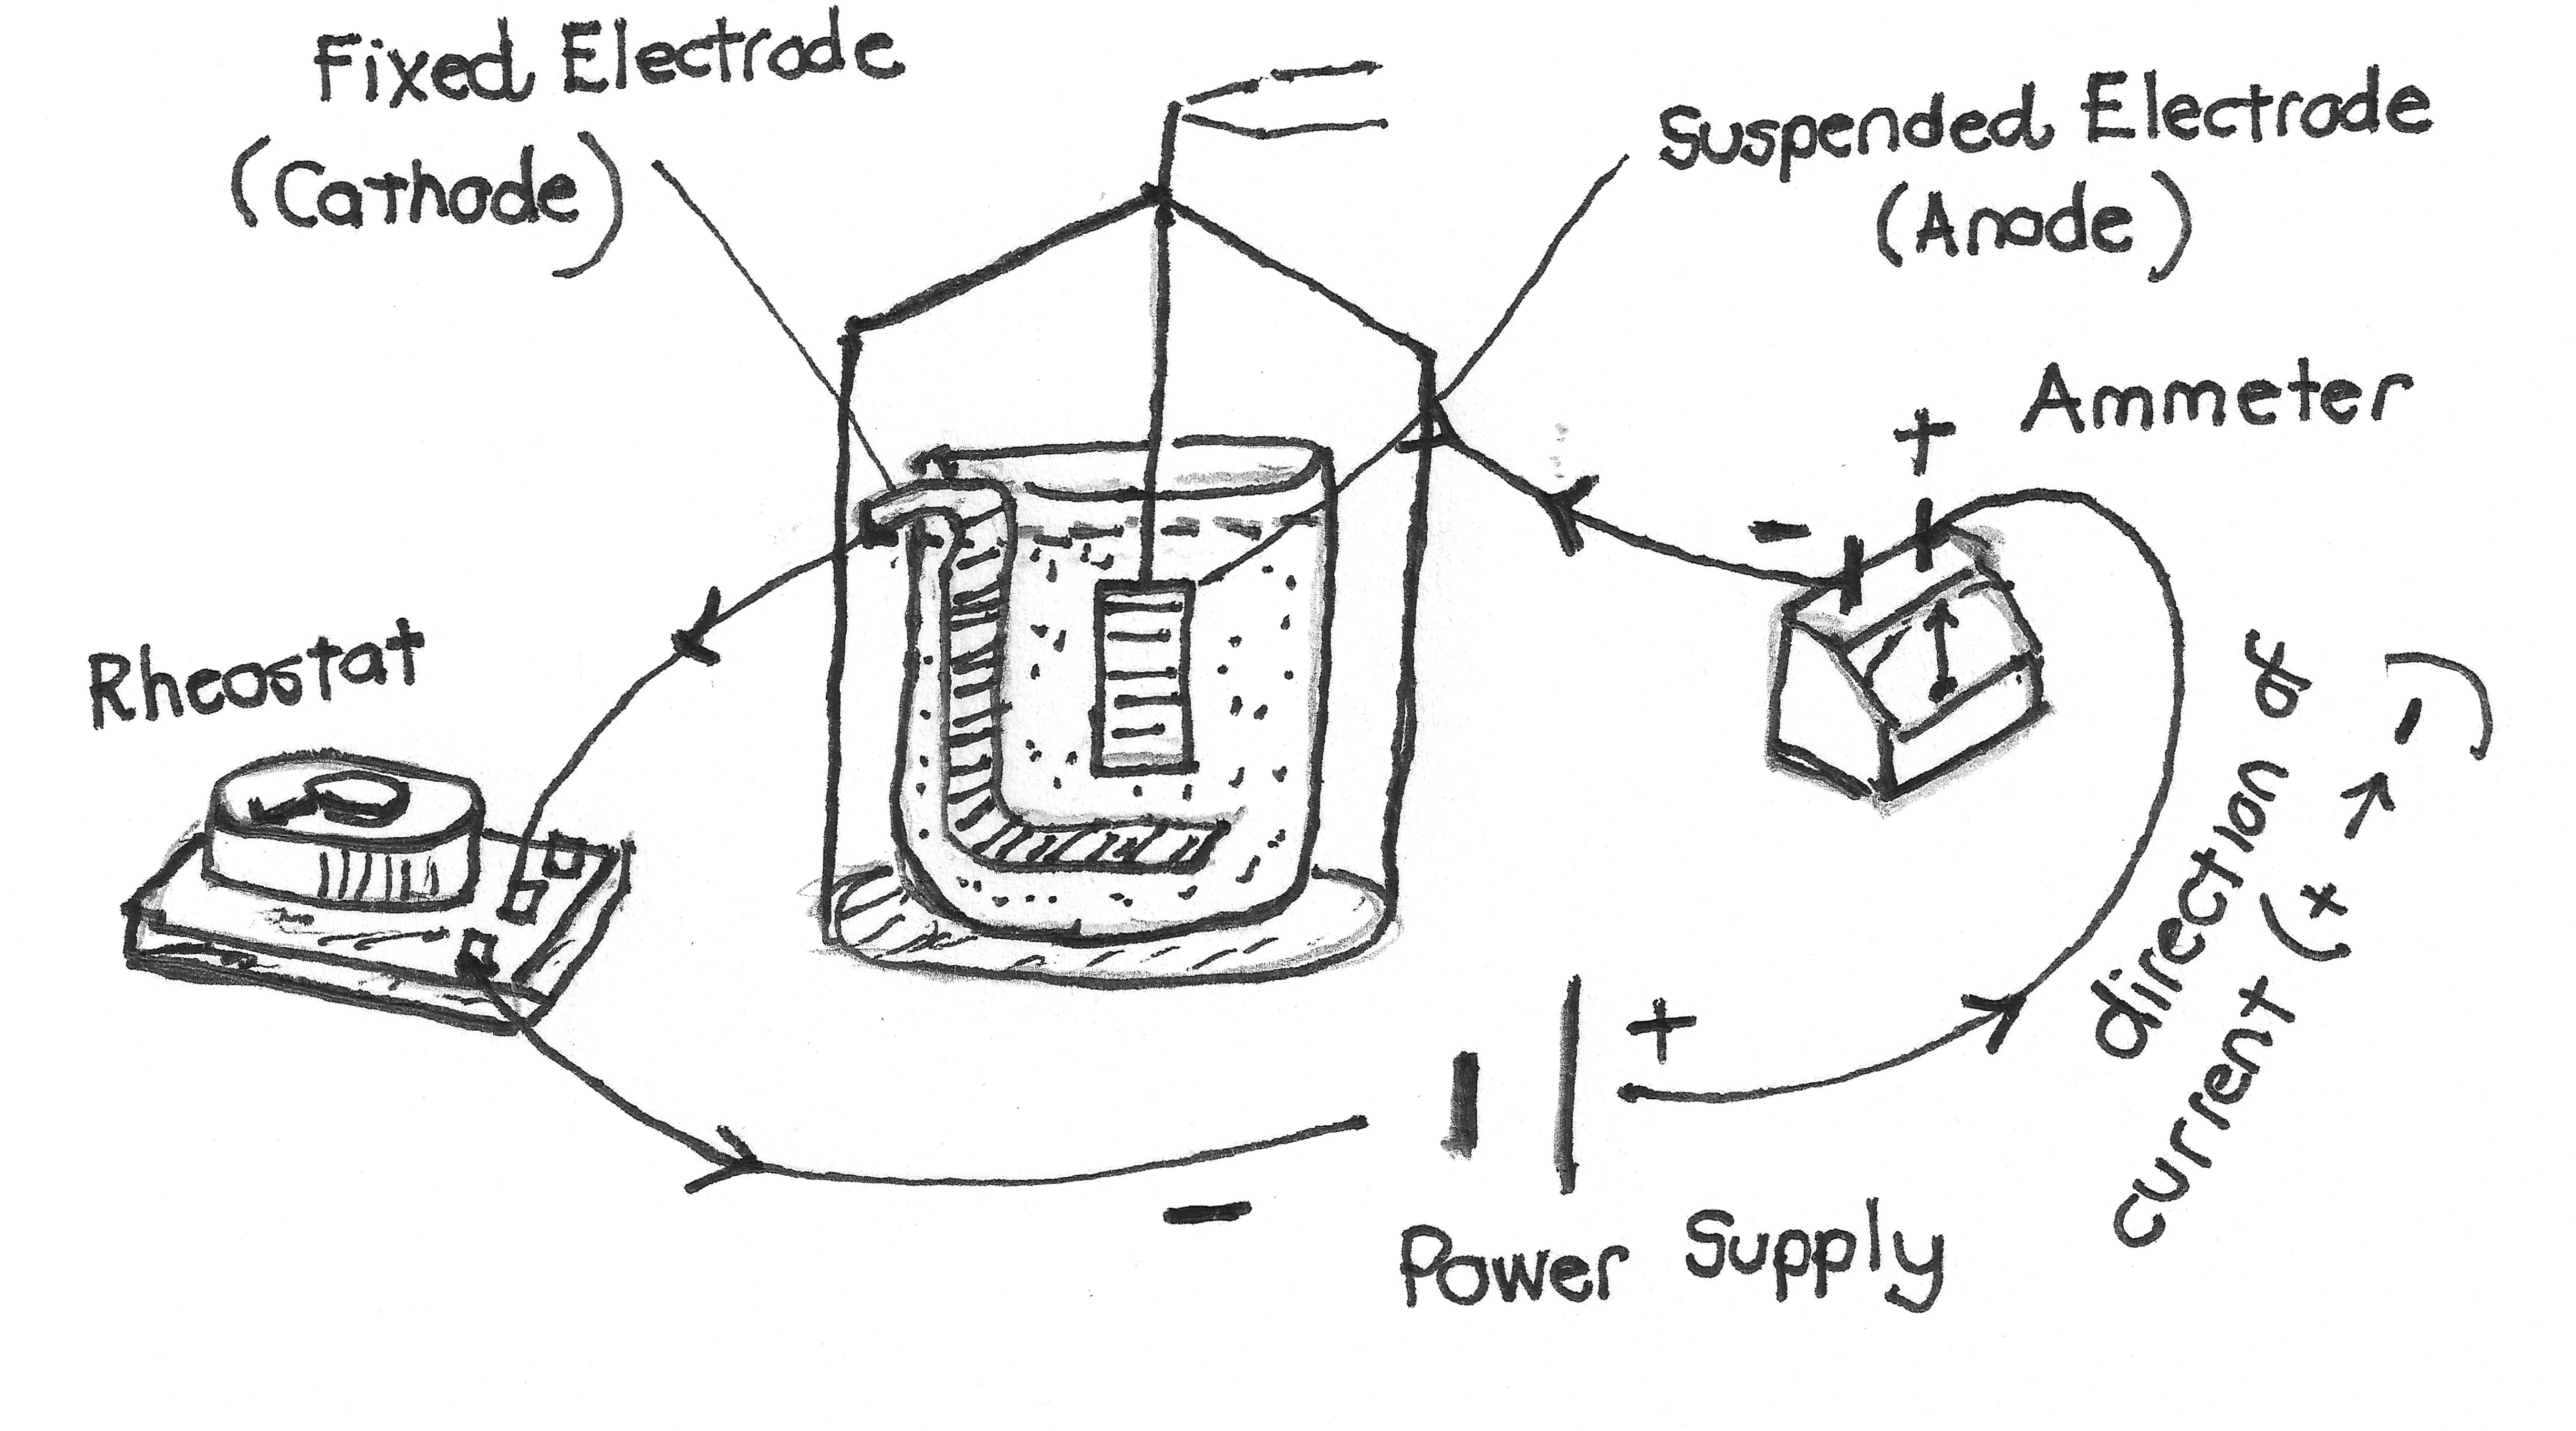
\includegraphics[width=4.88403in,height=2.20694in]{images/01_faraday/image003.png}
\caption*{\emph{With this wiring, the suspended copper electrode is an anode; the
fixed copper electrode a cathode. Copper is lost at the anode and gained at the cathode.
To reverse anode and cathode, run the current from the power
supply in the reverse directions, remembering that current in the
ammeter runs from positive (terminal) to negative.}}
\end{figure}

The plate to be weighed will be suspended directly from a metal stand.
The beaker, containing the electrolyte solution and the fixed electrode,
rests on the workbench. The fixed electrode is cut from a strip of pure
copper sheet and is about 1 inch wide; it must be long enough to run
along the bottom of the beaker.\footnote{This is to establish an
  electric field on both sides of the suspended plate; otherwise the
  action may be slow or erratic.} It should be bent to fit the edge of
the beaker and guided far enough away from the suspended plate to
prevent accidental contact.

Weigh both plates on the electronic balance. Then fit the fixed plate
into the beaker, and adjust the length of the suspension hook so that
the suspended plate can swing freely without touching the fixed plate.
You will have to make at least two plating trials.

Some groups will attach the spring clips---as suggested in the 
sketch---others will reverse them. Attach the fixed plate to the desired pole of
the power supply.

Next clip the remaining power supply lead to the fixed electrode. Start
a stopwatch as you turn on the power supply, and quickly bring the
current to some value between 1 and 2 amperes.\footnote{Don't waste time
  trying to target a "round number." In this age of pocket calculators,
  round numbers carry no advantage whatever. It is not important that
  the current have any particular value, but that it be \emph{steady}.}
During the run, continually adjust the rheostat to maintain a uniform
current through the solution.\footnote{Note that our rheostat
  illustrates the very technique Faraday mentioned in his note 3 
  above for using a fine (and hence high-resistance) wire as a current
  regulator!} In order to transfer an amount of material that will be
large compared with the sensitivity of the balance, it is best to plate
for at least 20 minutes if a 1-ampere current is used, at least 10
minutes if a 2-ampere current is used. Longer times give greater
precision of measurement, since the weights of material transferred are
then larger in relation to the uncertainty of the weight mea\-sure\-ments.

At the conclusion of the first timed run, turn off the power and remove
the beam clip and the electrical connection to the pan. Gently remove
the suspended electrode and dry it with a hair dryer before measuring
its change in weight.

Carry out a second run similar to the first. It is not necessary to keep
either the current or the plating time the same as before.

We are now in a position to investigate two relations which Faraday
observed to hold in electrolysis:

\subsection{Proportionality Between Weight and Charge for a Single Element}

According to Faraday, the quantity of charge that is supplied to an
electrochemical reaction during any time will be directly proportional
to the quantity of material de\-com\-posed (or transferred) in that time. We
first attempt to exhibit that proportionality.

Calculate the \emph{weight} of material transferred to or from the
weighing plate during the first run, and cumulatively over both runs.

Calculate the quantity of \emph{charge} passed during the first run, and
cumulatively over both runs:
\begin{equation*}
\text{Charge in coulombs = uniform current in amperes $\times$ time in seconds}
\end{equation*}

If the expected proportionality holds, the weight of material
transferred during the first run will be to the total weight transferred
as the charge calculated for the first plating is to the total charge
passed. Do the weights have to one another the same ratio as the
calculated charges?

\subsection{The Ratio of Charge to Weight for Multiple Elements}

We have, it is hoped, observed in electrolysis a constant relation
between charge and weight for a single element. But as Faraday also
described, the weights of two or more elements liberated or transferred
by the same quantity of charge are to one another in the same ratio as
their \emph{chemically equivalent weights}. Or, differently expressed,
\emph{the ratio between charge and equivalent weight is the same for all
elements.}

Faraday recognized this constant proportion, but he could not express it
in terms of a conventional unit of charge since at that time no such
standard had been defined.\footnote{Hence his recourse to such
  expressions as: ``sufficient to keep a platinum wire red hot,'' ``more
  than any man would willingly allow to pass through his body at once,''
  ``thirty turns of a very large and powerful plate machine.''} Using a
modern unit, it has subsequently been determined that a charge of about
96,500 coulombs\footnote{See the Appendix (p.~\pageref{ch:appendix})
for information about the various systems of measurement of electrical quantities.} 
is required to liberate one gram-equivalent weight of any element. That
quantity, 96,500 C, was named the \emph{faraday} in that
investigator's honor. The mea\-sure\-ments we have already taken in
electrodeposition of copper will permit us to calculate the faraday for
ourselves.

For we found in that experiment that a charge $Q$ was required to
transfer $\Delta W$ of copper. Now 1 faraday, $F$, is the charge
required to transfer one gram-equivalent weight of copper---31.78 g.
But the charges are to one another as the weights, as presumably we have
just confirmed; therefore
\begin{equation*}
Q : F :: \Delta W : 31.78\; \text{grams}.
\end{equation*}

Or, expressed algebraically,
\begin{equation*}
F = \frac{31.78\cdot Q}{\Delta W}.
\end{equation*}

Thus the faraday will equal the product of the charge passed in any run
of the electrodeposition experiment, times the gram-equivalent weight of
copper, divided by the weight of copper deposited in that run.

As we shall see, the actual size of the faraday---that is, the quantity
of charge found to be associated with one gram-equivalent weight of an
element in electrolysis---will become pivotal in some speculations which
J.\ J.\ Thomson allows himself in his paper that follows.

(It is, as Faraday himself keenly appreciated, extremely large: two
one-faraday charges placed one kilometer apart---if it were possible to do
this---would e\-lec\-tro\-stat\-ic\-al\-ly attract each other with a force of
\emph{trillions} of pounds.)
